%************************************************
\chapter{Development}
\label{ch:Development}
%************************************************



This chapter details the development phases of the battery health prediction system, covering the complete progress from initial MATLAB modeling to advanced deep learning implementation. The project evolved through distinct phases: (1) MATLAB-based modeling and simulation using traditional methods, (2) exploration of hybrid neural network approaches, (3) transition to pure data-driven models, and (4) implementation of state-of-the-art deep learning architectures for time series forecasting.

The development process was guided by the need to create accurate, strong, and scalable battery health prediction models capable of handling real-world applications. Each phase built upon lessons learned from previous approaches, ultimately leading to the implementation of TimesNet, a cutting-edge time series analysis architecture that demonstrates superior performance in battery degradation prediction tasks.

\section{MATLAB Modeling and Simulation}
\label{sec:matlab_modeling}

\color{Red}senti falta de uma ou duas figuras nesta secção. Uma com o Modelo Matlab Implementado e outra com o diagrama de blocos do Modelo da Batemo (mesmo que não possa mostrar valores por questões de confidencialidade do modelo a qeteve acesso ) \color{Black}

The initial development phase focused on implementing traditional battery modeling approaches in MATLAB to establish baseline performance and understand the basic characteristics of battery degradation patterns.

The exploration began with the MATLAB Simulink Battery State-of-Charge Estimation example~\cite{mathworks_battery_soc_2024} to evaluate the feasibility of generating synthetic battery data through simulation and to test the Kalman filter approach for state estimation. This standard example provided a foundation for understanding how battery behavior could be modeled and simulated using established MATLAB tools. Figure~\ref{fig:simulink_ekf_implementation} shows the complete MATLAB Simulink implementation used for Extended Kalman Filter testing and battery state estimation.

\begin{figure}[htbp]
\centering
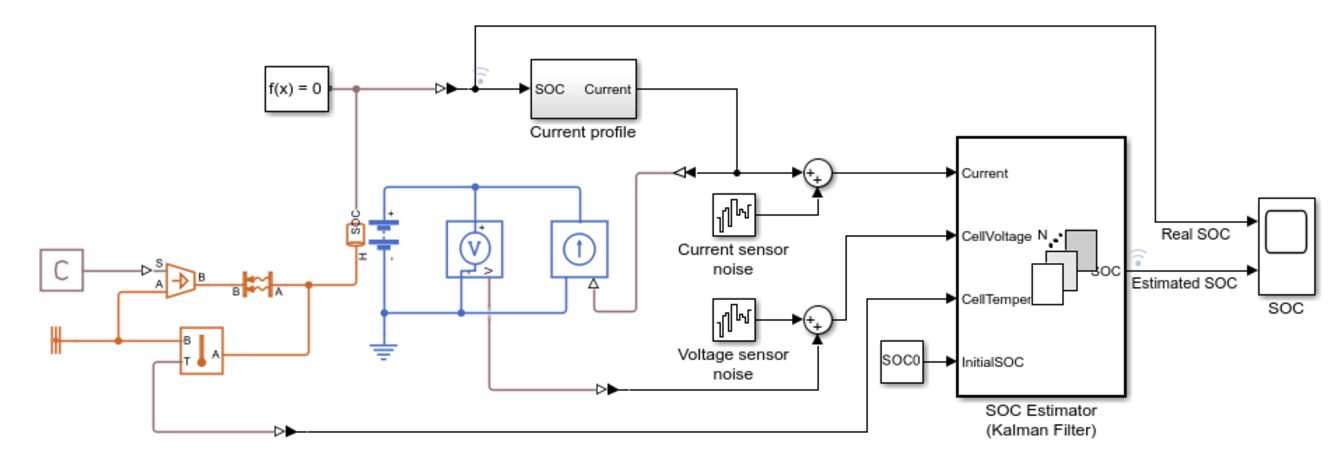
\includegraphics[width=0.9\textwidth]{imgs/simulink_EKF.png}
\caption{MATLAB Simulink implementation of Extended Kalman Filter for battery state-of-charge estimation, showing the complete simulation framework used for testing and validation.}
\label{fig:simulink_ekf_implementation}
\end{figure}

To enhance the accuracy and realism of the simulations, the standard battery block was replaced with the Batemo INR21700-p45b model, which was accessible through the Formula Student team collaboration at the polytechnic. The Batemo model~\cite{batemo_website_2024} offers a highly accurate, physics-based battery simulation with its own dedicated Simulink block, enabling more realistic testing conditions and validation of the proposed approaches. Figure~\ref{fig:batemo_blocks} illustrates the block diagram structure of the Batemo battery model integration within the simulation framework.

\begin{figure}[htbp]
\centering
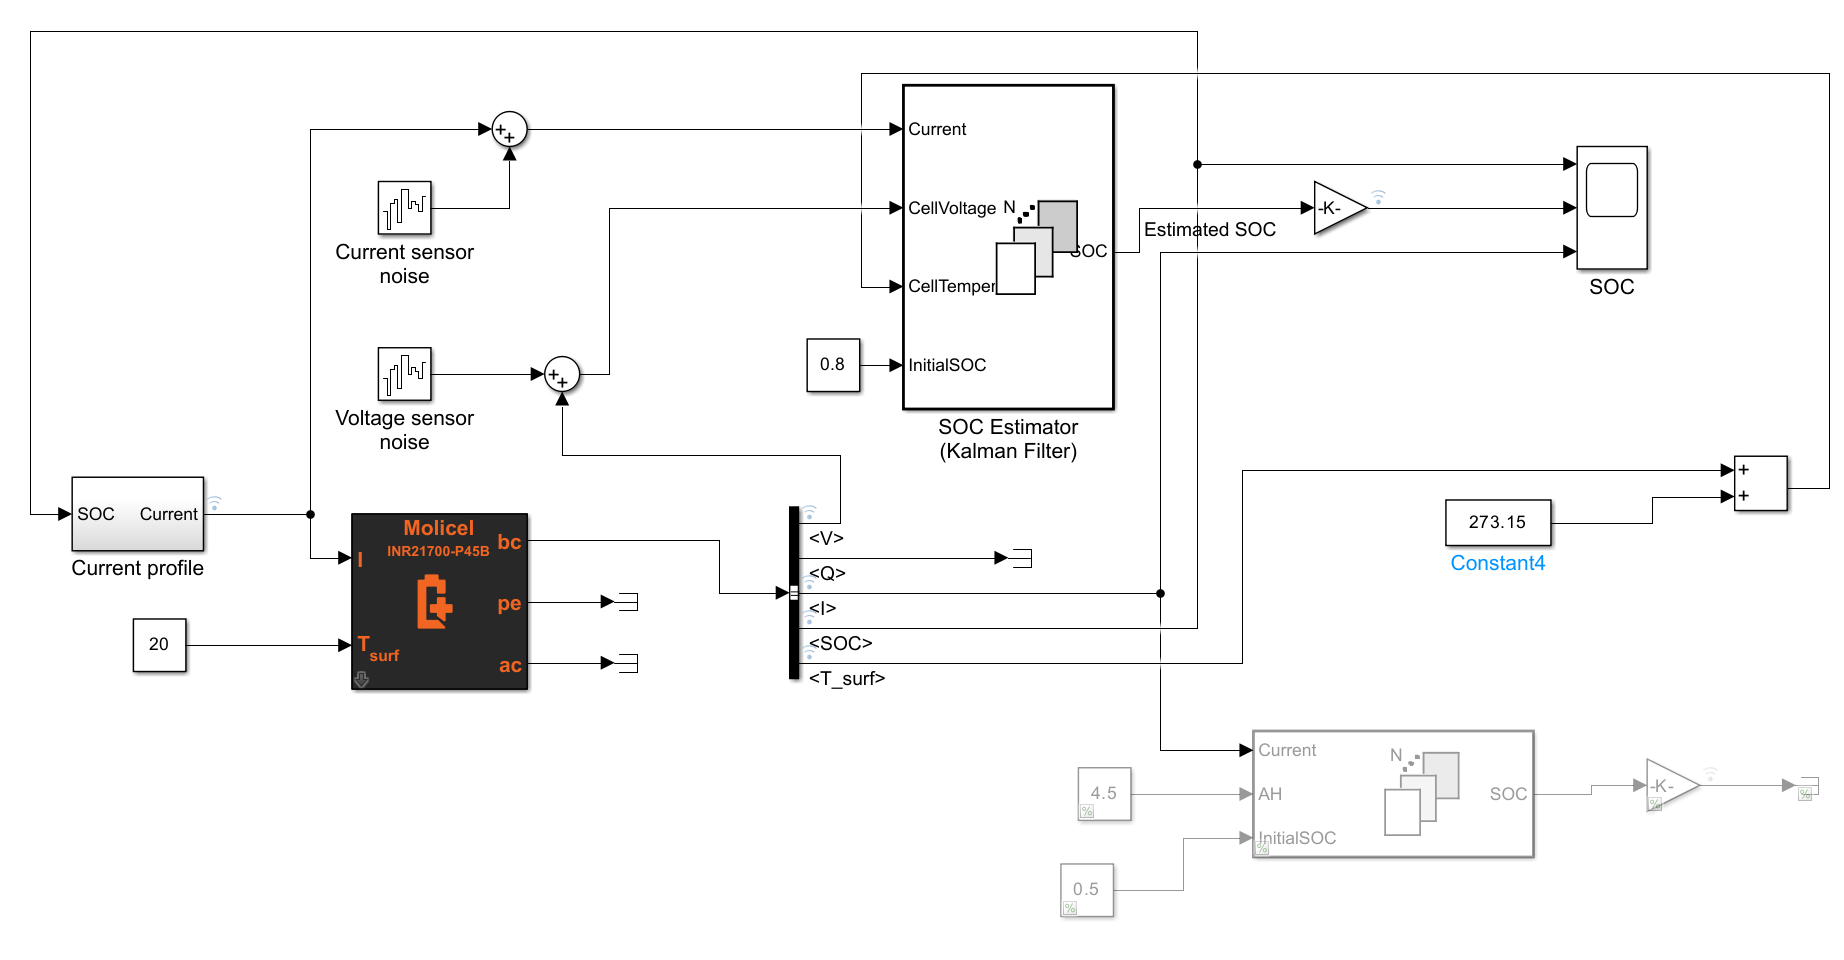
\includegraphics[width=0.8\textwidth]{imgs/batemo_blocks.png}
\caption{Block diagram of the Batemo INR21700-p45b battery model integration, showing the physics-based simulation structure used for enhanced accuracy in battery behavior modeling.}
\label{fig:batemo_blocks}
\end{figure}

First, the Extended Kalman Filter (EFK) was implemented as the primary estimation algorithm for SOC prediction. The EFK approach was chosen for its proven effectiveness in handling the nonlinear behavior of battery systems and its ability to provide uncertainty measurement. Coulomb counting was integrated as a supporting method for SOC estimation, providing a reference baseline for comparison with the Kalman filter results. Figure~\ref{fig:ekf_results} presents the estimation results obtained from the EKF implementation, demonstrating the algorithm's performance in tracking battery state-of-charge.

\begin{figure}[htbp]
\centering
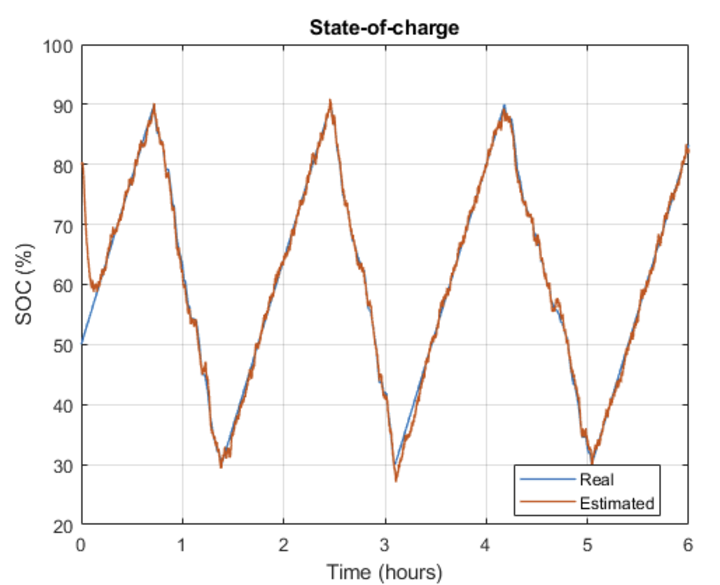
\includegraphics[width=0.9\textwidth]{imgs/EKF_results.png}
\caption{Extended Kalman Filter estimation results showing SOC tracking performance and comparison with reference measurements, illustrating the accuracy and reliability of the implemented algorithm.}
\label{fig:ekf_results}
\end{figure} 

The implementation addressed several critical considerations to ensure accuracy and reliability. \textbf{Current integration accuracy and drift compensation} were prioritized to minimize cumulative errors that could significantly impact SOC estimates over extended periods. \textbf{Temperature effects on coulombic efficiency} were carefully analyzed, as thermal variations can substantially alter the charge-discharge efficiency and affect the accuracy of capacity calculations. \textbf{Aging effects on capacity estimation} were incorporated to account for the gradual degradation of battery capacity over operational lifetime, ensuring that SOC estimates remain accurate as the battery ages. Finally, \textbf{calibration procedures for initial SOC determination} were established to provide accurate baseline measurements, which are crucial for the cumulative nature of coulomb counting methods.

The Batemo battery model was incorporated to provide physics-based battery behavior simulation. This integration offered complete capabilities for model development and validation. Figure~\ref{fig:batemo_configurations} shows the detailed configuration options available in the Batemo model, while Figure~\ref{fig:batemo_estimation} demonstrates the estimation capabilities achieved through the physics-based simulation approach.

\begin{figure}[htbp]
\centering
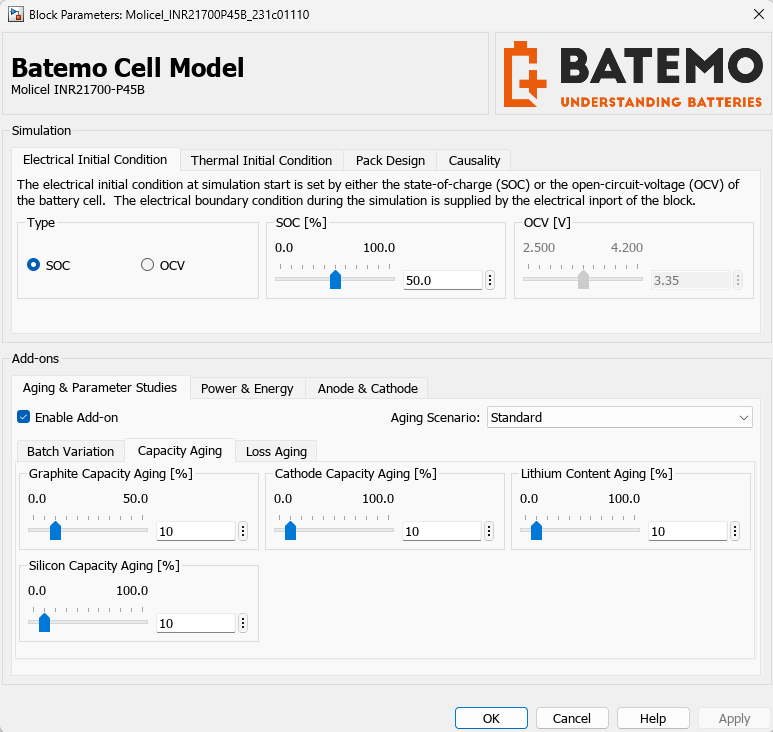
\includegraphics[width=0.8\textwidth]{imgs/batemo_configurations.png}
\caption{Batemo battery model configuration interface, showing the various agging and batterry parameters}
\label{fig:batemo_configurations}
\end{figure}

\begin{figure}[htbp]
\centering
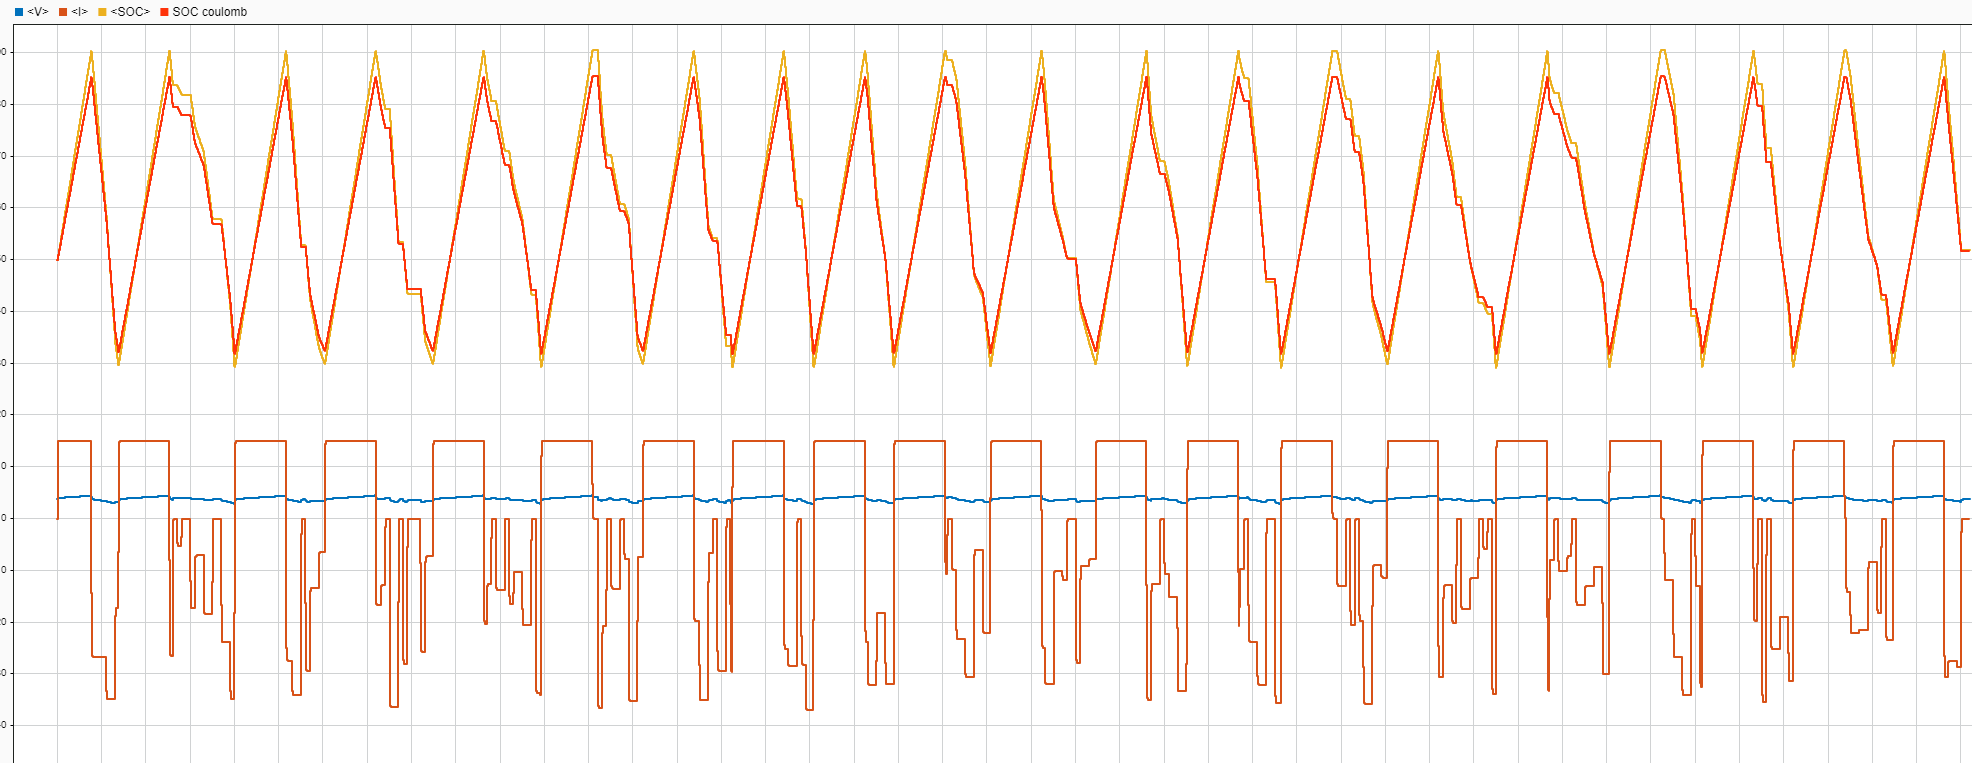
\includegraphics[width=0.9\textwidth]{imgs/batemo_estimation.png}
\caption{Battery state estimation results obtained using the Batemo physics-based model, demonstrating improved accuracy compared to standard battery models. The top graph shows the estimated SOC (orange line) compared with the actual SOC (yellow line).}
\label{fig:batemo_estimation}
\end{figure}

\textbf{Validation of estimation algorithms under controlled conditions} was enabled through the model's ability to simulate precise battery behaviors, allowing for systematic testing of algorithm performance across various operational scenarios. \textbf{Generation of synthetic data for algorithm testing} provided a valuable resource for training and evaluating neural networks when real-world data was limited or when specific degradation patterns needed to be studied. \textbf{Analysis of model sensitivity to various degradation mechanisms} was made possible by the physics-based nature of the Batemo model, enabling detailed investigation of how different aging phenomena affect battery performance predictions. Additionally, \textbf{comparison between model-based and data-driven approaches} was made possible, allowing for complete evaluation of different estimation methodologies and their respective strengths and limitations.

This MATLAB implementation served as a foundation for understanding battery dynamics and provided insights that informed subsequent neural network development phases. The experience gained from working with both simulated and physics-based models highlighted the importance of high-quality data and the potential benefits of combining model-based insights with data-driven approaches.

\section{Neural Network Approaches}
\label{sec:neural_network_evolution}

This work evaluated different NN approaches, each addressing specific limitations identified in others and incorporating lessons learned from the MATLAB modeling phase.

%\subsection{Hybrid (CNN + LSTM) Architecture}
%\label{subsec:cnn_lstm_architecture}
%
%The first neural network implementation combined CNN with LSTM networks to leverage both spatial feature extraction and temporal sequence modeling capabilities\color{Red}Referencia da rede que usou\color{Black}. This CNN+LSTM architecture was structured to use the supporting strengths of both convolutional and recurrent neural networks. The design incorporated multiple specialized layers, each serving a distinct purpose in the feature extraction and temporal modeling pipeline.\color{Red}Ficava bem a referência a uma figura que mostrasse o diagrama de blocos da arquitetura\color{Black} \textbf{CNN layers} were responsible for extracting local patterns and features from battery measurement sequences, identifying spatial relationships and important signal characteristics within the input data. \textbf{LSTM layers} focused on modeling long-term dependencies and temporal relationships, capturing the sequential nature of battery degradation and state evolution over time. Finally, \textbf{Dense layers} provided the final prediction mapping with appropriate activation functions, transforming the processed features into accurate SOC and SOH estimates.
%
%Several significant challenges were encountered during the implementation that highlighted the complexity of applying deep learning to battery health monitoring. These obstacles required careful analysis and ultimately influenced the decision to pursue alternative approaches. \textbf{Gradient vanishing} emerged as a critical issue where long sequences caused training instability, preventing the network from effectively learning long-term dependencies essential for accurate battery state prediction. \textbf{Overfitting} presented another major concern, as the high model complexity led to poor generalization, with the network memorizing training patterns rather than learning transferable features applicable to new battery data. \textbf{Computational efficiency} posed practical limitations, with training time becoming too long for large datasets, making the approach unsuitable for real-world applications requiring timely model updates. Additionally, \textbf{Feature engineering} proved challenging, as manual feature selection proved suboptimal, requiring extensive domain expertise and iterative refinement that limited the model's adaptability to different battery types and operating conditions.
%
%\subsection{Hybrid vs. Data-Driven Approach Evaluation}
%\label{subsec:hybrid_vs_datadriven}
%
%A systematic comparison was conducted between hybrid approaches (combining physics-based models with neural networks) and pure data-driven methods.\color{Red}Tem de dizer que modelos experimentou em cada uma das abordagens, indicando referências e apresentando figuras \color{Black}
%
%The hybrid approach integrated multiple supporting techniques to use both physics-based understanding and data-driven learning capabilities. This complete strategy incorporated several key components designed to enhance prediction accuracy and reliability. \textbf{Physics-based model outputs as additional input features} provided domain-specific insights that enriched the neural network's understanding of battery behavior, incorporating basic electrochemical principles into the learning process. \textbf{Kalman filter estimates as regularization terms} helped constrain the neural network training by incorporating well-established state estimation techniques, reducing the likelihood of unrealistic predictions and improving model stability. Furthermore, \textbf{domain knowledge constraints in loss function design} ensured that the learned models respected known physical limitations and relationships, preventing the network from learning patterns that violated basic battery physics principles.
%
%The pure data-driven approach emphasized maximum use of machine learning capabilities while minimizing reliance on explicit domain knowledge. This methodology focused on allowing the neural network to discover patterns and relationships directly from the data. \textbf{End-to-end learning from raw sensor data} enabled the model to process unfiltered battery measurements, potentially capturing subtle patterns that might be lost during manual preprocessing or feature engineering steps. \textbf{Automatic feature extraction and representation learning} allowed the network to identify the most relevant characteristics for battery health prediction without requiring extensive domain expertise or manual feature design. Additionally, \textbf{minimal domain-specific preprocessing requirements} reduced implementation complexity and improved the method's adaptability to different battery types and measurement configurations, making it more suitable for diverse real-world applications.
%
%The evaluation revealed that data-driven approaches demonstrated \textbf{better generalization} across different battery chemistries, \textbf{reduced dependency} on accurate physics model parameters, \textbf{better scalability} to large datasets, and \textbf{more strong performance} under varying operating conditions. This analysis motivated the transition to advanced pure data-driven architectures, which require the use of comprehensive and high-quality datasets.

\subsection{Transformer and Mixture of Experts Networks}
\label{subsec:transformer_moe_networks}

During the literature review process, the Transformer network for Remaining Useful Life prediction of lithium-ion batteries by Chen et al. (2022) \cite{chen_transformer_2022} was identified as a promising approach that demonstrated superior performance for battery health prediction tasks. This work introduced a Transformer-based neural network specifically designed for battery RUL prediction using the CALCE dataset \cite{CALCE_battery_nodate}.

The Chen et al. approach addressed the challenge of noisy battery capacity data through a two-stage framework. First, a Denoising Auto-Encoder (DAE) was applied to process the raw battery data and reduce noise artifacts commonly present during charge-discharge cycles. The denoised data was then fed into a Transformer network to capture temporal information and learn features relevant to battery degradation patterns. The unified framework combined both denoising and prediction tasks, enabling end-to-end learning for accurate RUL estimation.

The Transformer architecture utilized self-attention mechanisms to model long-range dependencies in battery degradation sequences, effectively capturing relationships between distant time points in the battery operational history. This approach demonstrated superior performance compared to traditional methods on multiple battery datasets, showing improved accuracy in predicting both State of Health (SOH) and End of Life (EOL) estimates. Figure~\ref{fig:transformer_architecture} illustrates the complete Transformer architecture implemented for battery RUL prediction, showing the multi-head attention mechanisms and feed-forward layers that enable effective temporal pattern recognition.

\begin{figure}[htbp]
\centering
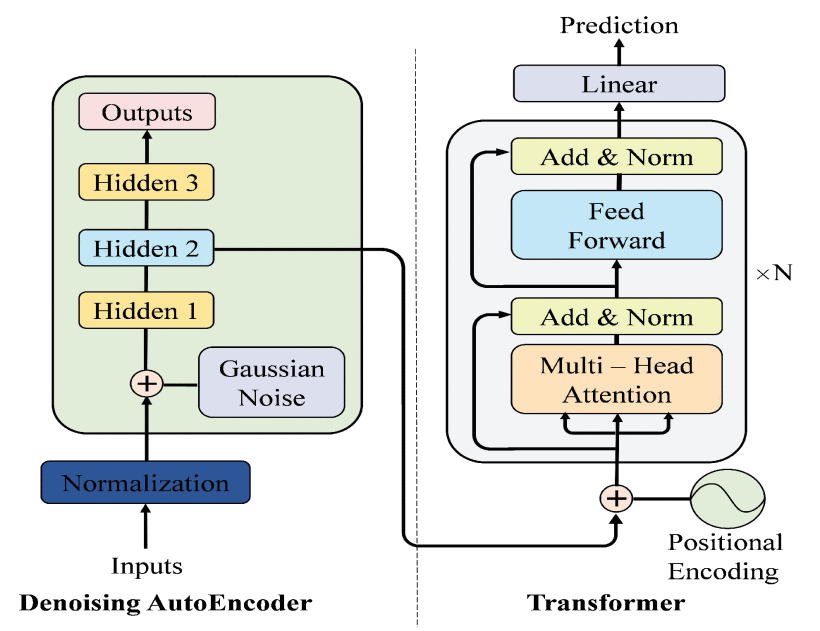
\includegraphics[width=0.9\textwidth]{imgs/transformer_arq.png}
\caption{Transformer architecture for battery RUL prediction, showing the self-attention mechanisms and encoder-decoder structure that enables modeling of long-range dependencies in battery degradation sequences\cite{chen_transformer_2022}.}
\label{fig:transformer_architecture}
\end{figure}

Building on concepts from Transferred Multi-Task Learning \cite{che_battery_2023}, which showed promise for battery state monitoring across different operating conditions, an investigation into Mixture of Experts (MoE) networks was conducted. MoE represents a powerful neural network architecture that combines multiple specialized sub-networks (experts) with a gating mechanism that determines which experts should be activated for each input sample.

The MoE architecture offers several advantages for battery health prediction:

\begin{itemize}
    \item \textbf{Specialized learning}: Different experts can focus on specific battery degradation modes or operating conditions
    \item \textbf{Computational efficiency}: Only a subset of experts are activated for each prediction, reducing computational overhead
    \item \textbf{Feature-specific tuning}: Experts can be optimized for different input features (voltage, current, temperature)
    \item \textbf{Scalable capacity}: Model capacity can be increased by adding experts without proportional computational cost increase
\end{itemize}

To evaluate the effectiveness of MoE networks for battery RUL prediction, the same experimental setup as the Chen et al. Transformer paper was replicated, but with the Transformer architecture replaced by a MoE network. The MoE implementation consisted of three specialized experts and a learned gating network that dynamically weighted expert contributions based on input characteristics. Figure~\ref{fig:moe_architecture} presents the detailed architecture of the implemented MoE network, highlighting the gating mechanism and expert specialization that enables efficient and targeted learning for different aspects of battery behavior.

\begin{figure}[htbp]
\centering
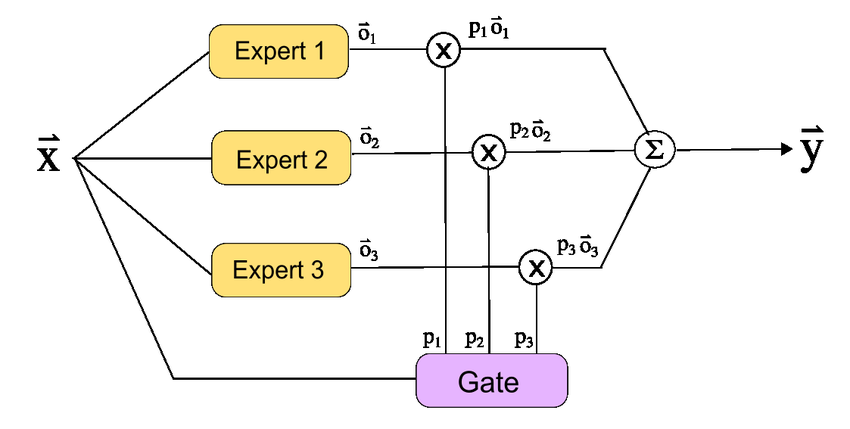
\includegraphics[width=0.9\textwidth]{imgs/Moe_arq.png}
\caption{Mixture of Experts (MoE) architecture for battery health prediction, showing the gating network and specialized experts that enable efficient learning of different battery degradation patterns and operating conditions~\cite{moe_arq}.}
\label{fig:moe_architecture}
\end{figure}

% Transformer results figure
\begin{figure}[htbp]
    \centering
    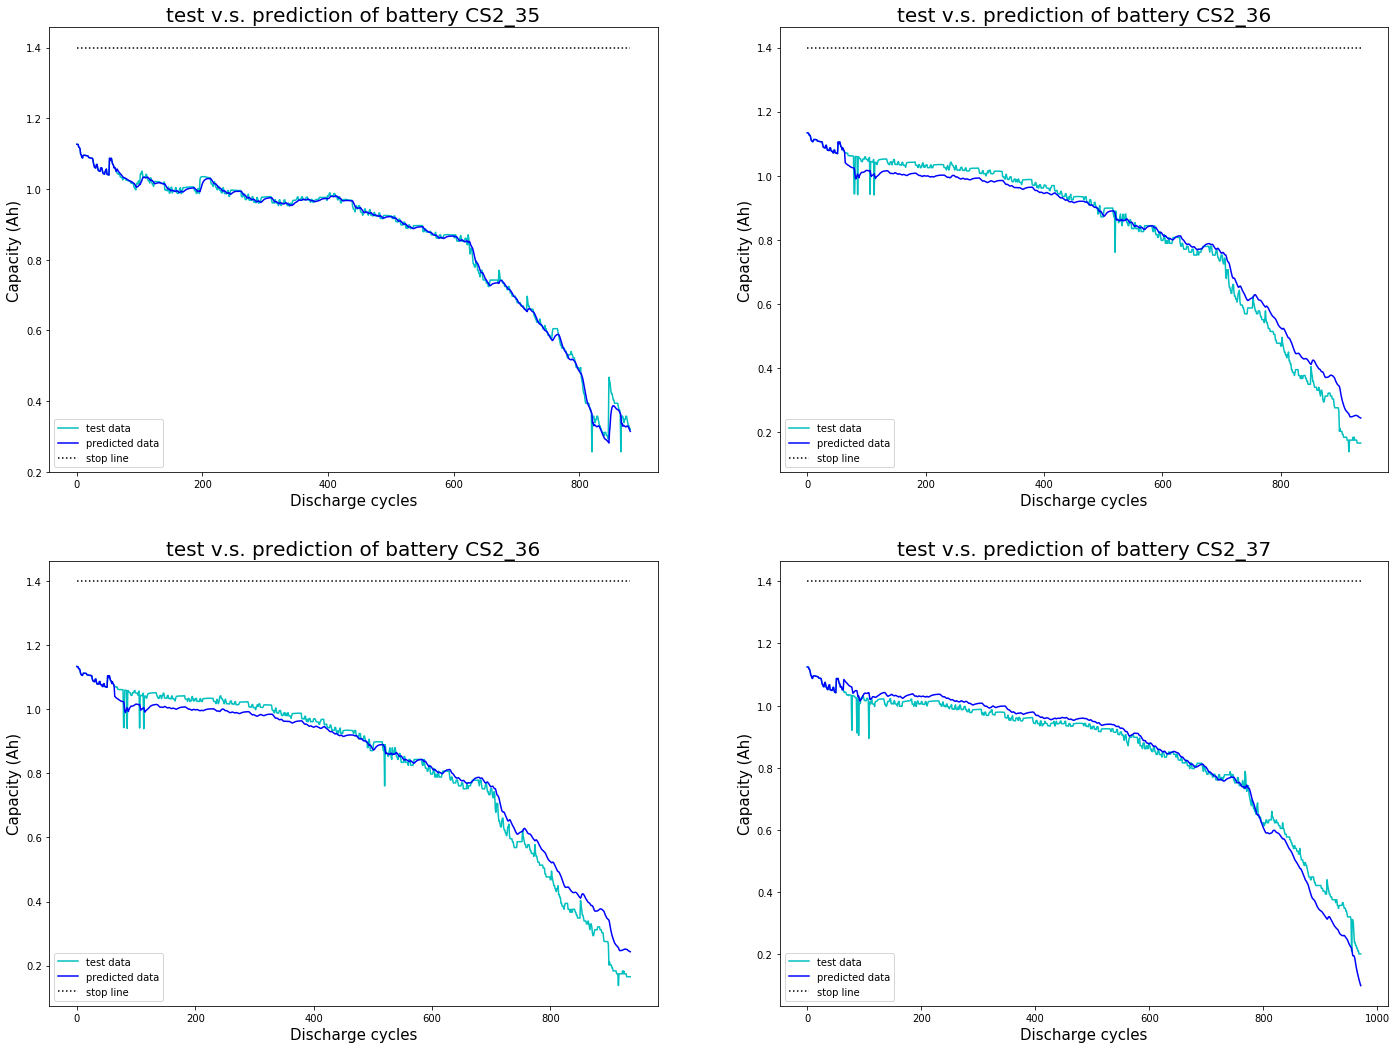
\includegraphics[width=0.9\textwidth]{imgs/transf_graph_results.png}
    \caption{Transformer network performance results for battery RUL prediction on CALCE dataset, showing prediction accuracy and convergence behavior during training and validation phases.}
    \label{fig:transformer_results}
\end{figure}

% MoE results figure
\begin{figure}[htbp]
    \centering
    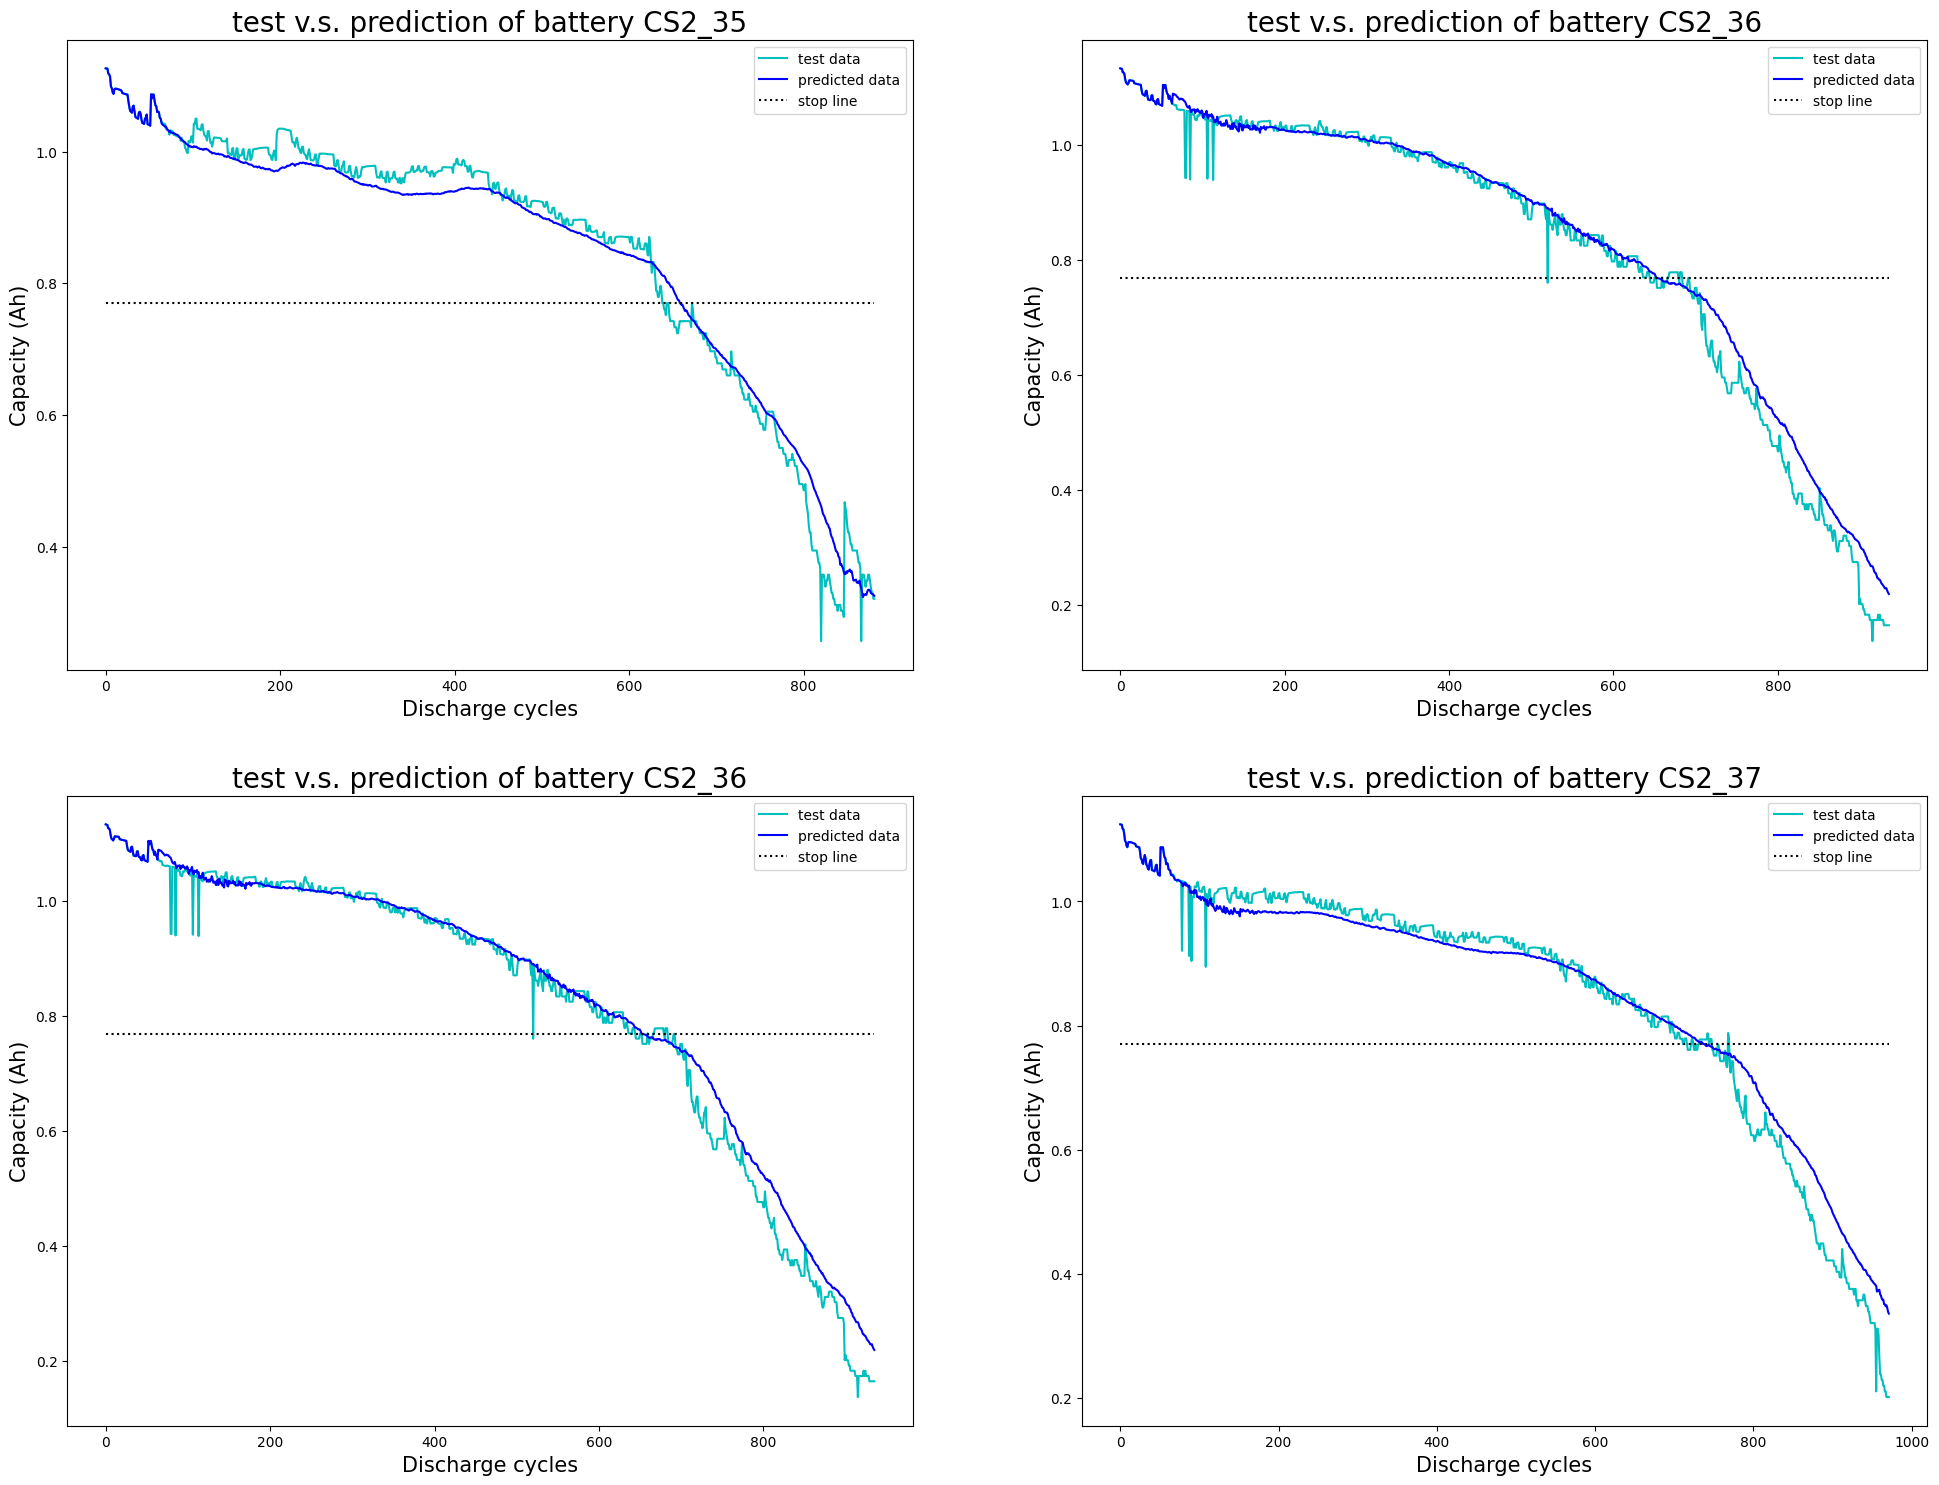
\includegraphics[width=0.9\textwidth]{imgs/moe_graph_results.png}
    \caption{Mixture of Experts (MoE) network performance results for battery RUL prediction, demonstrating competitive accuracy with reduced computational complexity compared to the Transformer approach.}
    \label{fig:moe_results}
\end{figure}

\begin{table}[htbp]
    \centering
    \caption{Quantitative comparison of Transformer vs. MoE network performance for battery RUL prediction}
    \label{tab:transformer_moe_results}
    \begin{tabular}{lc}
        \hline
        \textbf{Model} & \textbf{RMSE} \\
        \hline
        Transformer & 0.0297 \\
        FCN MoE & 0.0335 \\
        \hline
    \end{tabular}
\end{table}

The experimental results demonstrated that a simple MoE network with just three experts could achieve performance levels comparable to the much more complex Transformer-based architecture. Figure~\ref{fig:transformer_results} shows the training and validation performance of the Transformer network, while Figure~\ref{fig:moe_results} presents the corresponding results for the MoE implementation. Table~\ref{tab:transformer_moe_results} provides a quantitative comparison of the two approaches, showing that while the Transformer model achieved a slightly better Root Mean Square Error (RMSE) of 0.0297 compared to the FCN MoE network's 0.0335, the MoE network provided competitive results with significantly reduced model complexity and computational requirements.

The MoE approach proved particularly effective due to its ability to specialize different experts for distinct aspects of battery behavior. Expert analysis revealed that the three experts naturally specialized in different degradation phases: early battery life, linear degradation, and end-of-life behavior. This specialization allowed the MoE network to capture the complex multi-phase nature of battery degradation with a simpler overall architecture.

This experiment demonstrated the potential of MoE networks as an efficient alternative to complex Transformer architectures for battery health prediction tasks, offering a good balance between prediction accuracy and computational efficiency.

\section{Dataset Collection and Preprocessing}
\label{sec:dataset_preprocessing}

The dataset development process was crucial for training strong and generalizable models, requiring careful consideration of data quality, diversity, and preprocessing strategies. Before selecting the final dataset, a comprehensive study of available battery datasets was conducted to evaluate their suitability for battery health prediction tasks.

\subsection{Dataset Comparison and Selection}
\label{subsec:dataset_comparison}

Multiple publicly available battery datasets were analyzed and compared based on their features, data completeness, and relevance to battery health prediction tasks. Table~\ref{tab:dataset_comparison} presents a comprehensive comparison of the evaluated datasets, highlighting the available features and characteristics of each dataset.

\begin{table}[htbp]
\centering
\caption{Comparison of available battery datasets and their features}
\label{tab:dataset_comparison}
\resizebox{\textwidth}{!}{%
\begin{tabular}{lcccccccccccccccc}
\hline
\textbf{Dataset} & \textbf{Cell Type} & \textbf{Chemistry} & \textbf{Time} & \textbf{C/D Ind.} & \textbf{Cycle} & \textbf{Current} & \textbf{Voltage} & \textbf{Dis. Cap.} & \textbf{Ch. Cap.} & \textbf{Ch. Energy} & \textbf{Dis. Energy} & \textbf{dV/dt} & \textbf{Int. Res.} & \textbf{AC Imp.} & \textbf{ACI Phase} & \textbf{Temp.} \\
\hline
Zn-ion, Na-ion @2025 & Various & Zn-ion, Na-ion & $\checkmark$ & $\checkmark$ & & $\checkmark$ & $\checkmark$ & $\checkmark$ & $\checkmark$ & & & & & & & \\
CALCE CS2 @2010 & Prismatic & LiCoO2 & $\checkmark$ & $\checkmark$ & $\checkmark$ & $\checkmark$ & $\checkmark$ & $\checkmark$ & $\checkmark$ & $\checkmark$ & $\checkmark$ & $\checkmark$ & $\checkmark$ & $\pm$ & $\pm$ & Initial \\
MATR @2019 & 18650 & LFP/graphite & $\checkmark$ & $\checkmark$ & $\checkmark$ & $\checkmark$ & $\checkmark$ & $\checkmark$ & $\checkmark$ & $\checkmark$ & $\checkmark$ & $\checkmark$ & $\checkmark$ & & & $\checkmark$ \\
MATR @2019 CL & 18650 & LFP/graphite & $\checkmark$ & & $\checkmark$ & $\checkmark$ & $\checkmark$ & $\checkmark$ & $\checkmark$ & $\checkmark$ & $\checkmark$ & $\checkmark$ & & & & $\checkmark$ \\
HUST @2022 & Various & LFP/graphite & $\checkmark$ & $\pm$ & $\checkmark$ & $\checkmark$ & $\checkmark$ & $\checkmark$ & $\checkmark$ & & & & & & & \\
RWTH @2017 & 18650 & Lithium Ion & $\checkmark$ & $\checkmark$ & $\checkmark$ & $\checkmark$ & $\checkmark$ & $\checkmark$ & $\checkmark$ & $\checkmark$ & $\checkmark$ & & & & & $\checkmark$ \\
ISU-ILCC @2023 & 502030 & Li-polymer & $\checkmark$ & & & $\checkmark$ & $\checkmark$ & $\checkmark$ & $\checkmark$ & $\checkmark$ & $\checkmark$ & & & & & \\
XJTU @2022 & 18650 & NCM Li-ion & $\checkmark$ & & & $\checkmark$ & $\checkmark$ & $\checkmark$ & $\checkmark$ & & & & & & & $\checkmark$ \\
Tongji @2022 & 18650 & NCA/NCM & $\checkmark$ & & $\checkmark$ & $\checkmark$ & $\checkmark$ & $\checkmark$ & $\checkmark$ & & & & & & & \\
Stanford @2024 & 21700 & Graphite/Si & $\checkmark$ & & $\checkmark$ & $\checkmark$ & $\checkmark$ & $\checkmark$ & $\checkmark$ & $\checkmark$ & $\checkmark$ & $\checkmark$ & $\checkmark$ & & & $\checkmark$ \\
\hline
\end{tabular}}
\end{table}

The evaluation considered several critical factors for battery health prediction applications:

\begin{itemize}
    \item \textbf{Data completeness}: Availability of essential measurements including voltage, current, capacity, and temperature
    \item \textbf{Temporal coverage}: Complete cycle life data spanning from beginning of life to end of life
    \item \textbf{Documentation quality}: Well-documented experimental conditions and measurement procedures
    \item \textbf{Research adoption}: Established use in the battery research community for benchmarking
    \item \textbf{Data quality}: Consistent sampling rates and minimal measurement artifacts
\end{itemize}

Based on this comprehensive analysis, the CALCE (Center for Advanced Life Cycle Engineering) battery dataset~\cite{CALCE_battery_nodate}, obtained from the University of Maryland's public repository, was selected as the primary dataset for this work. This dataset was selected for its:

\begin{enumerate}
    \item Complete cycle life data spanning multiple battery chemistries
    \item High-quality measurements with consistent sampling rates
    \item Well-documented experimental conditions and procedures
    \item Established use in battery research community for benchmarking
\end{enumerate}


Several preprocessing steps were implemented to ensure data quality and model training stability, namely:

\begin{itemize}
    \item \textbf{Initial cycle removal}: The first charge-discharge cycle was removed from each battery file to avoid initialization artifacts and inconsistent starting conditions
    \item \textbf{Incomplete cycle filtering}: Cycles with insufficient data points or incomplete charge/discharge sequences were excluded from the training set
    \item \textbf{Outlier detection}: Statistical methods were applied to identify and remove measurement outliers that could negatively impact model training
\end{itemize}

Battery-level partitioning was also employed to prevent data leakage, ensuring that cycles from the same battery appeared in only one partition. The input data structure was then designed to optimize model performance, using the following techiques:

\begin{itemize}
    \item \textbf{Sequence length}: Fixed-length sequences of 100 time steps were extracted from continuous battery operation data.
    \item \textbf{Feature vector}: Each time step included voltage, current, temperature, and derived features such as power and energy.
    \item \textbf{Target variables}: State of Health (SOH) values were calculated based on capacity fade measurements.
    \item \textbf{Sliding window}: Overlapping sequences were generated to maximize training data utilization.
\end{itemize}

\section{Selected Deep Learning Approach}
\label{sec:timesnet_model}

The evaluation of CNN+LSTM and hybrid approaches revealed several critical limitations:

\begin{itemize}
    \item \textbf{Temporal modeling constraints}: Traditional LSTM architectures struggled with very long sequences typical in battery degradation analysis
    \item \textbf{Multi-scale pattern recognition}: Difficulty in capturing both short-term fluctuations and long-term degradation trends simultaneously
    \item \textbf{Computer efficiency}: High computer requirements limited the scalability to large datasets
    \item \textbf{Generalization issues}: Poor performance when applied to battery chemistries or operating conditions not seen during training
\end{itemize}

The identified requirements for an improved architecture included:

\begin{itemize}
    \item \textbf{Multi-periodicity detection}: Ability to automatically identify and exploit multiple periodic patterns in battery data
    \item \textbf{Long-range dependency modeling}: Effective capture of dependencies across extended time horizons
    \item \textbf{Parameter efficiency}: Reduced model complexity while maintaining or improving performance
    \item \textbf{Versatility}: Capability to handle various time series analysis tasks beyond just forecasting
\end{itemize}

These requirements led to the selection and implementation of TimesNet, a cutting-edge architecture specifically designed for general time-series analysis.bTimesNet is a modern neural network designed specifically for analyzing time series data~\cite{wu_timesnet_2023}. This model tackles the basic challenge of understanding how data changes over time by converting the complex problem from analyzing 1D time series into analyzing 2D patterns.\color{Red}devia fazer aqui referência ao diagrama de blocos da rede e apresenta-la numa figura. Pode ser aqui ou mais à frente, mas devia aparecer. \color{Black} The key innovation of TimesNet is its ability to discover repeating patterns (periodicity) in time series data and break down complex time changes into smaller, more manageable pieces.


TimesNet starts by analyzing the time series in the frequency domain using FFT to discover multiple periods. Real-world time series usually present multi-periodicity, such as daily and yearly variations for weather observations, or weekly and quarterly variations for electricity consumption. The period discovery process works by analyzing the frequency spectrum of the input data. The algorithm calculates the amplitude of different frequencies and identifies the strongest periodic patterns by selecting the top-k frequencies with the highest amplitudes. These dominant frequencies correspond to the most important periodic behaviors in the data, such as charge-discharge cycles in battery operations or longer-term capacity fade patterns.


The architecture works by converting 1D time series into a set of 2D grids based on multiple identified periods. This transformation organizes patterns within each period into columns and patterns across different periods into rows of the 2D grids, making time patterns easier to analyze using 2D image processing techniques. Based on the selected frequencies and corresponding period lengths, the 1D time series is reshaped into multiple 2D tensors. This process takes the original time series data and reorganizes it into a grid-like format where each period becomes a row and the progression through different periods becomes columns.

The reshaping process essentially converts temporal patterns into spatial patterns that can be analyzed using 2D image processing techniques. Each identified period creates a separate 2D representation of the data, allowing the model to examine patterns at different time scales simultaneously.
Figure~\ref{fig:timesnet_2d_transformation} illustrates this transformation process, showing how discovering periodicity enables the conversion of original 1D time series into structured 2D tensors that can be processed by 2D kernels conveniently. 

\subsection{TimesBlock Architecture}

The core component, TimesBlock, can automatically discover multiple periods and extract complex time patterns using efficient inception blocks. Each TimesBlock works in a way that preserves the original signal while adding new information, and consists of two main parts:

\begin{enumerate}
\item \textbf{Capturing time patterns in 2D}: After converting the 1D time series into multiple 2D grids, each grid is processed by an efficient inception block that uses different sized filters. This design allows the model to examine patterns at multiple scales - both within individual periods (columns) and across different periods (rows) at the same time.

\item \textbf{Adaptive aggregation}: The k different processed features are combined based on their corresponding amplitudes of the estimated periods. The model uses a weighted combination where stronger periodic patterns (higher amplitudes) have more influence on the final result. This adaptive weighting ensures that the most important temporal patterns dominate the model's predictions.
\end{enumerate}

The shared inception block design makes the model size stay the same regardless of how many periods k are selected, improving efficiency.

\begin{figure}[htbp]
    \centering
    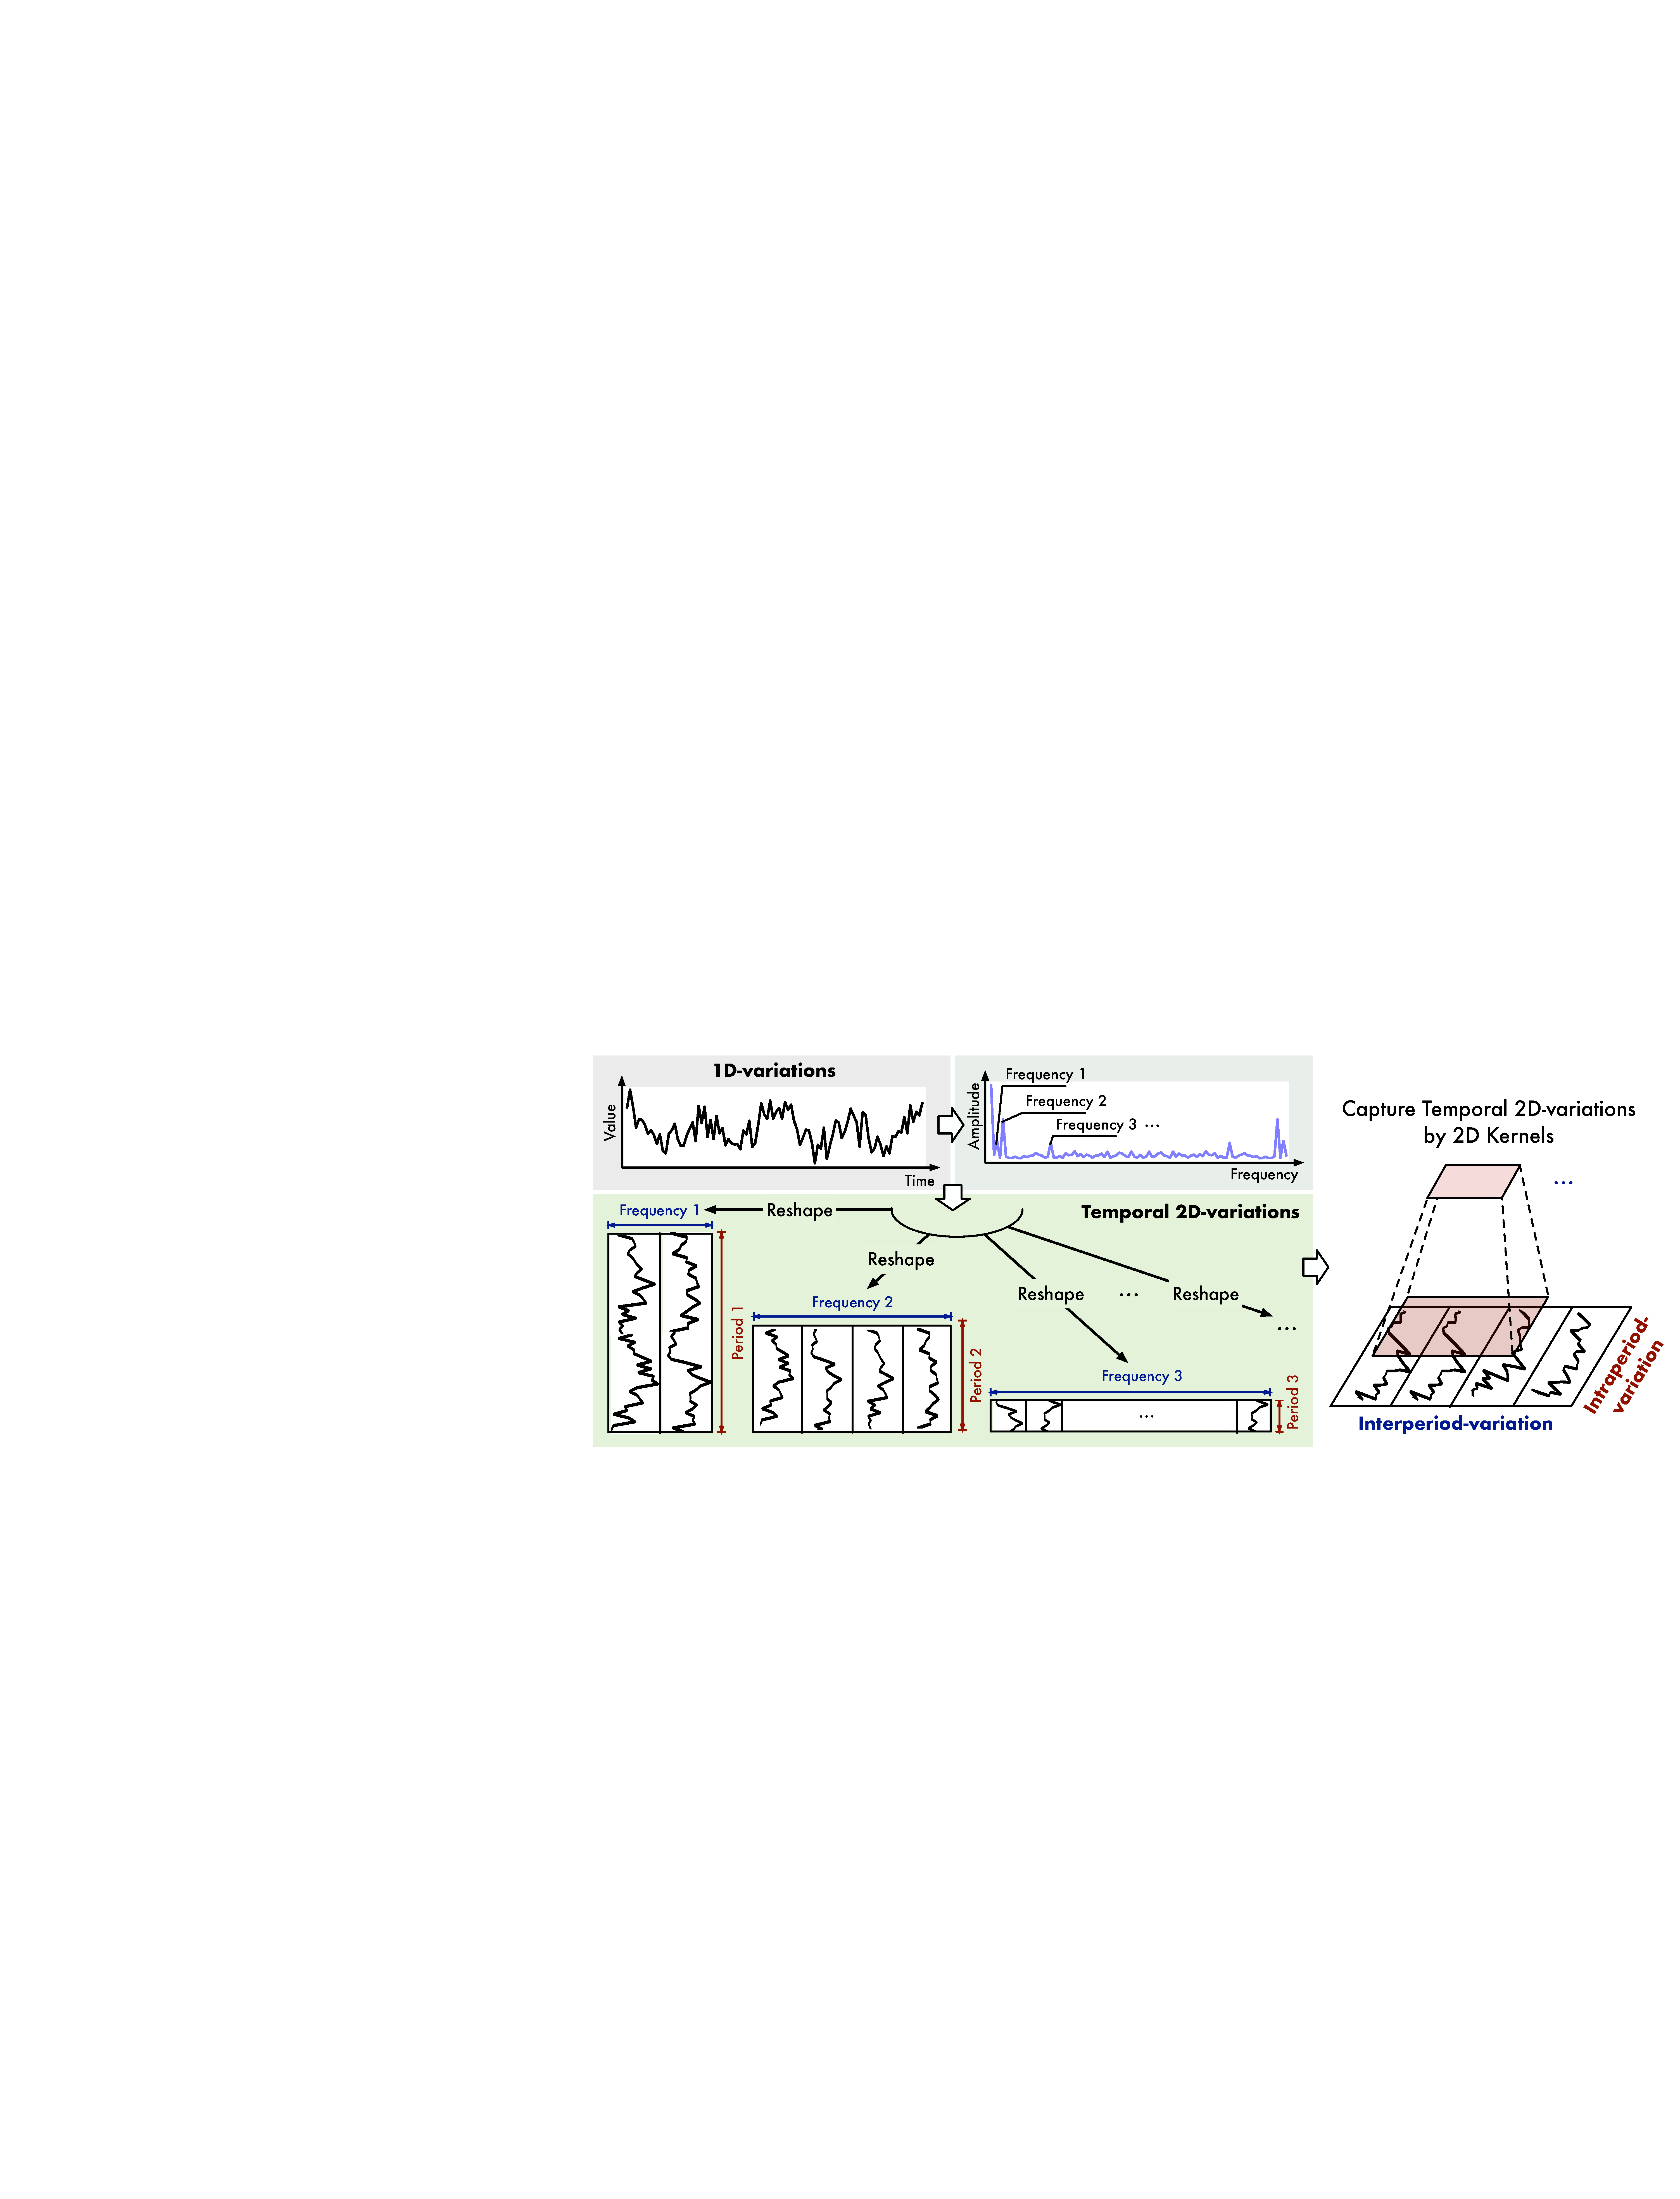
\includegraphics[width=1.0\textwidth]{imgs/timesnet_2d_structure.pdf}
    \caption{TimesNet 2D transformation: converting 1D time series into structured 2D tensors by discovering periodicity~\cite{wu_timesnet_2023}.}
    \label{fig:timesnet_2d_transformation}
\end{figure}

TimesNet shows better performance across five main time series analysis tasks: short-term and long-term forecasting, filling in missing data, classification, and anomaly detection. This flexibility makes it particularly suitable for battery health prediction tasks, where complex time dependencies and patterns at multiple scales are crucial for accurate state-of-health estimation. 

The model's ability to handle various sequence lengths and its strong design for capturing time dynamics work well with the requirements of battery degradation modeling, where both short-term changes and long-term trends must be considered at the same time. Key advantages include:

\begin{itemize}
\item \textbf{Multi-scale time modeling}: The 2D transformation allows capturing both short-term battery behavior (within periods) and long-term degradation trends (across periods) at the same time.
\item \textbf{Automatic period detection}: The FFT-based period discovery can identify natural cycles in battery operation without manual setup.
\item \textbf{Efficiency}: The shared inception block design keeps the model compact while handling multiple time scales.
\item \textbf{Flexibility}: The general-purpose nature allows adaptation to different battery types and operating conditions.
\end{itemize}

Unlike previous methods that struggle with the complex time patterns in battery data, TimesNet's 2D approach makes time changes easier to analyze. The transformation breaks the limitation of representation ability in the original 1D space, enabling more effective modeling of complex battery degradation patterns. The TimesNet architecture was therefore adapted for battery health prediction with several key modifications to optimize performance for this specific domain:

\begin{itemize}
    \item \textbf{Input preprocessing}: Battery measurement sequences (voltage, current, temperature) were formatted to exploit the multi-periodicity detection capabilities. The input sequences were structured to capture both charge-discharge cycles and longer-term aging patterns.
    \item \textbf{Output configuration}: Modified for regression tasks to predict continuous SoH values rather than classification outputs. The final layer was adapted to output single scalar values representing battery health percentages.
    \item \textbf{Loss function}: Used Mean Squared Error (MSE) with additional rules to prevent overfitting and ensure stable training.
    \item \textbf{Feature engineering}: Minimal manual feature creation to use the model's automatic pattern discovery abilities. This approach allows TimesNet to automatically identify relevant time patterns in battery data without requiring specialized feature design.
    \item \textbf{Period selection}: The top-k parameter was optimized specifically for battery data characteristics, allowing the model to focus on the most relevant repeating patterns in battery operation and degradation cycles.
\end{itemize}

\subsection{Model Optimization}
\label{sec:model_optimization}

TimesNet implementation followed the general framework with battery-specific optimizations:

\begin{itemize}
    \item \textbf{Sequence length}: Fixed-length sequences of 100 time steps were used to capture sufficient temporal context while maintaining computational efficiency.
    \item \textbf{Period discovery}: The FFT-based period detection was applied to identify natural cycles in battery operation, such as charge-discharge patterns and longer-term capacity fade cycles.
    \item \textbf{2D tensor processing}: The inception blocks were configured with appropriate kernel sizes to capture multi-scale temporal variations relevant to battery degradation processes.
    \item \textbf{Aggregation weights}: The amplitude-based aggregation mechanism was used to automatically weight different periodic components based on their importance in the frequency domain.
\end{itemize}

\subsection{Hyperparameter Search}

For model optimization, the Optuna tool was utilized, which enables hyperparameter optimization for machine learning models, integrated with Weights \& Biases (WandB), which allows for result visualization and model comparison. The dataset was reduced to only 1/10 of the data, equally distributed from the original dataset, with the objective of reducing the time required for finding the best hyperparameters, since this process took approximately one week even with this data reduction.

For the hyperparameter search, 50 trials were performed, with 50 epochs each, using an early stopping patience of 5 epochs to avoid overfitting and accelerate the optimization process. The parameters that were optimized through Optuna are:

\begin{itemize}
    \item \textbf{e\_layers}: Number of encoder layers (1--3) --- controls the depth of the encoder stack
    \item \textbf{d\_layers}: Number of decoder layers (1--3) --- controls the depth of the decoder stack  
    \item \textbf{factor}: Expansion factor for the FFN (1--5) --- controls the complexity of frequency components in TimesNet
    \item \textbf{freq}: Frequency for time features encoding (``s'', ``t'', ``h'') --- seconds, minutes, hours
    \item \textbf{d\_model}: Model dimension (fixed at 16)
    \item \textbf{top\_k}: Top-k dominant frequencies in TimesNet (1--5) --- controls how many frequency components to consider
\end{itemize}

Through this optimization, it was possible to detect the importance of the hyperparameters. The analysis showed that the importance factor of the \textbf{e\_layers} parameter (number of encoder layers) is the parameter that most influences the result when changed, demonstrating that the depth of the encoder architecture is critical for model performance.

\textbf{Network Optimization Discussion}
\label{subsec:best_trial_results}

The most successful trial was trial 15, which presented the following results:

\begin{itemize}
    \item \textbf{MSE Value}: 0.0015545075293630362
    \item \textbf{Optimal Parameters}:
    \begin{itemize}
        \item e\_layers: 2
        \item factor: 4  
        \item d\_model: 16
        \item top\_k: 9
        \item n\_heads: 16
    \end{itemize}
    \item \textbf{Duration}: 7770232 ms (approximately 2 hours and 10 minutes)
\end{itemize}

The results show that using 2 encoder layers works better than deeper networks, likely avoiding overfitting on the battery dataset. The high expansion factor of 4 allows the model to capture more complex patterns, while setting top\_k to 9 means the model considers more frequency components than the default range, which helps capture the various periodic behaviors in battery degradation cycles.

\chapter{Experiments and Results}
\label{sec:experiments_results}

\lipsum[2-4]

\chapter{Conclusion and Future Work}
\label{sec:conclusion_future_work}
\lipsum[1]
\section{Conclusion}
\lipsum[5-6]
\section{Future Work}
\lipsum[7-8]


